\section{Project Requirements}
\subsection{Software Requirements}
In order to reproduce the artefact, software requirements must be installed and hardware requirements must be met as prerequisites to the project. While some software, like the development environments are optional and are not needed to train the models, some modification to the code might be needed to run without them.

\phantomsection
\subsubsection{Python}
The entirety of the projects code was written in Python and such is a hard requirement to run the projects artefact. It is recommended to use Python 3.7 or later for TensorFlow support.

\subsubsection{TensorFlow and Keras}
The TensorFlow and Keras are used in the entirety of this project and such is a hard requirement to run the artefact. It is recommended to use TensorFlow 2.0 and Keras 2.0 or later, but with some code modifications, TensorFlow 1.0+ and Keras 1.0+ can also be used.

\subsubsection{TensorBoard}
In this project, TensorBoard 2.8.0 was used and is a hard requirement to run the artefact. As with TensorFlow, it is recommended to use TensorBoard 2.0 or later, but with some code modifications, TensorBoard 1.0+ can also be used.

\subsubsection{Scikit-Learn}
In this project, Scikit-Learn 1.0.2 was used and is a hard requirement to run the artefact.

\subsubsection{pandas}
In this project, pandas 1.3.5 was used and is a hard requirement to run the artefact.

\subsubsection{NumPy}
In this project, NumPy 1.21.6 was used and is a hard requirement to run the artefact.

\subsubsection{Google Cloud Platform - Development Environment}
Google Cloud Platform and its subsidiary solutions are not a requirement to run the artefact, however can be used to run model training simultaneously.

\subsubsection{Google Colab - Development Environment}
Google Colab is not a requirement to run the artefact, however a Jupyter notebook solution, like this, must be used.

\subsubsection{Project Code}
The project code is hosted on GitHub, and can be accessed and downloaded through the following link: \url{https://github.com/laurencebrwn/ml-covid19-eval}. The results and individual models notebook files are all found here.

\subsubsection{COVIDx-CXR Dataset}
The dataset used to train the image classification models is a hard requirement for this project. The full dataset is hosted on kaggle, and can be found here: \url{https://github.com/lindawangg/COVID-Net/blob/master/docs/COVIDx.md}. The images should be obtained from the "COVIDx CXR-2 Kaggle Dataset" link (\url{https://www.kaggle.com/datasets/andyczhao/covidx-cxr2}) detailed on the previously linked page. The labels for both binary ("train\_COVIDx9B.txt" and "test\_COVIDx9B.txt") and multi-label ("train\_COVIDx9A.txt" and "test\_COVIDx9A.txt") classification, can be downloaded from the link (\url{https://github.com/lindawangg/COVID-Net/tree/master/labels}) detailed on the previously linked page.

\subsection{Hardware Requirements}
While TensorFlow can run on a large number of devices, there are some hardware limitations, especially if a Graphical Processing Unit (GPU) is used to accelerate performance. TensorFlow requires a CPU capable of AVX instructions, which most modern Computational Processing Unit's (CPU) support \citep{InstallT17:online}. If GPU acceleration is required and the device used has an NVIDIA GPU, then it must support compute unified device architecture (CUDA), a "parallel computing platform" which can "dramatically speed up computing applications by harnessing the power of GPUs" \citep{CUDAZone2:online}. If the device has a GPU that does not support CUDA, but does support DirectX 12 (e.g. an AMD GPU manufactured in the last several years), then Microsoft's DirectML can be used enable GPU support for TensorFlow \citep{Introduc93:online}. Precautions must be taken if DirectML is used however, as it has differing version requirements of Python, TensorFlow and NumPy.

\section{Design}
In order to design the software that would train and evaluate each of the selected models, identified in the literature review, prompts were taken from the methodology to devise a structure that would form each models notebook. By implementing a general structure that all models would inherit, it made changes to the models, hyper parameters easy, while reducing development time. While there are a few variations for each model a common format was followed for all models:

\begin{enumerate}
    \item Set up the environment.
    \begin{enumerate}
        \item Define the model and training variables.
        \item Import the required libraries, like TensorFlow, Keras, Scikit-Learn, etc.
        \item Define the hyper-parameters of the model (or list of hyper-parameters if performing tuning).
    \end{enumerate}
    \item Prepare the dataset.
    \begin{enumerate}
        \item Read in the label files for both test and train.
        \item Down-sample each class to match the total dataset size and to ensure all classes are equally represented.
        \item Shuffle the data.
        \item Pre-process the X-Ray images (and perform image transformations on the training dataset).
        \item Split the training data into folds for stratified K fold cross validation.
    \end{enumerate}
    \item Create the machine learning model.
    \begin{enumerate}
        \item Create the Keras sequential model.
        \item If the model is using transfer learning (Xception, ResNet and DenseNet), fetch the base model from Keras' application library.
        \item Define the model layers in the sequential model.
        \item Set any hyper-parameters, like the optimiser, learning rate etc.
        \item Compile the model.
    \end{enumerate}
    \item Begin cross validation training.
    \begin{enumerate}
        \item Iterate through hyper-parameter variations.
        \item Iterate through stratified K folds.
        \item Train the model.
        \item Record model logs.
        \item Save the model weights.
    \end{enumerate}
    \item Evaluate the model.
    \begin{enumerate}
        \item Iterate through the trained models.
        \item Load model weights.
        \item Predict the labels on the test dataset.
        \item Record the models key metrics, described in the methodology.
        \item Save the models metrics and performance
    \end{enumerate}
\end{enumerate}

\section{Developing the Artefact}
Developing the Python notebooks for each model followed a similar flow to that listed in the design section. Firstly the Environment set up was developed, followed by dataset preparation and pre-processing. Where the development flow differed was that the cross validation training and evaluation sections were developed before the model itself. This meant a skeletal structure consisting of everything except for the model itself could be replicated, once for each model. This section will detail the development via a run through of the code itself, split into the sections listed in the flow above.

\subsection{Environment Set Up}
Firstly the correct environment had to be set up before any machine learning models were created or training was to happen. This started with defining the image size, batch size, dataset size, number of K folds, the maximum amount of epochs and the path to the dataset. Secondly all the required libraries were imported. This included NumPy, pandas, TensorFlow, Scikit-Learn, TensorBoard and other generic Python libraries like those used to record the time. Finally the hyper-parameters were instantiated. This was done using TensorBoard's "hparams" plugin. An example of this can be seen in \autoref{fig:hyper-param-code}.

\begin{figure}[H]
    \centering
    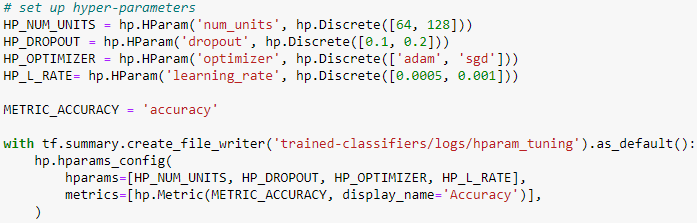
\includegraphics[width=\textwidth]{figures/hyper-param-code.png}
    \caption{Defining the hyper-parameters with TensorBoard.}
    \label{fig:hyper-param-code}
\end{figure}

\subsection{Dataset Preparation}
Next the COVIDx-CXR dataset had to be brought in, and manipulated such that the models could use it for training. To begin, the dataset labels were read in, and unnecessary columns, like "patient id" and "data source" were removed. Next the data was down-sampled, such that the classes were of equal proportions, and thoroughly shuffled. This was done with Scikit-Learns "resample" function, an example of this can be seen in \autoref{fig:dataset-downsampling}. 

\begin{figure}[H]
    \centering
    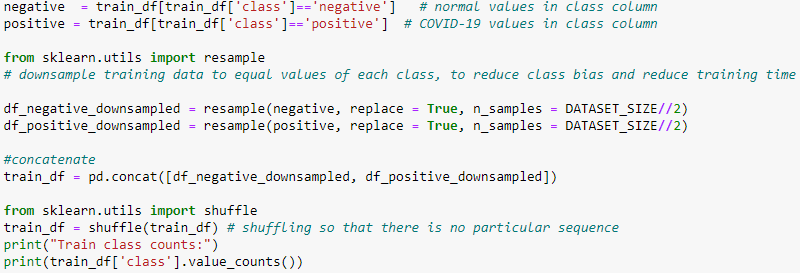
\includegraphics[width=\textwidth]{figures/dataset-downsampling.png}
    \caption{Down-sampling and shuffling the dataset.}
    \label{fig:dataset-downsampling}
\end{figure}

The dataset labels then had to be linked with the corresponding images. This was done with Keras' "ImageDataGenerator". Using "ImageDataGenerator" allowed for the use of the "flow\_from\_dataframe()" function, which matches up the image paths, stored in a DataFrame, to the images themselves. It also allowed for image pre-processing to be performed serially, each time an image was flowed from the DataFrame. While the image pre-processing remained mostly constant for each model, some models, like Xception, ResNet and DenseNet, each had a specific pre-processing, created for that model, by Keras. Pre-processing the training images also took a different form from the test images, as the data had to be split into training and validation folds, dictated by the stratified K fold implementation. A separate function was made for this purpose, an example of which, used for the Xception model, can be seen in \autoref{fig:image-preprocessing}.

\begin{figure}[H]
    \centering
    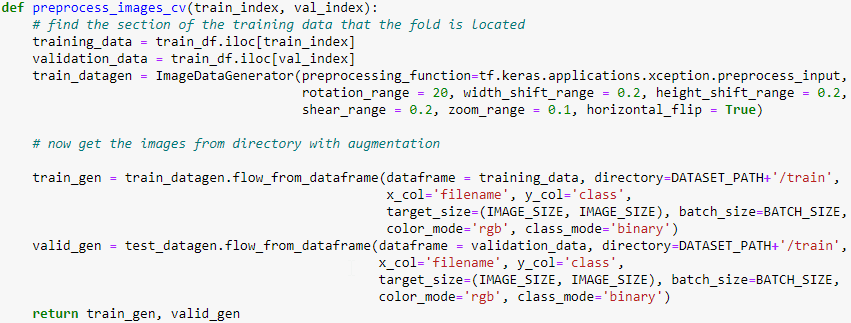
\includegraphics[width=\textwidth]{figures/image-preprocessing.png}
    \caption{Down-sampling and shuffling the dataset.}
    \label{fig:image-preprocessing}
\end{figure}

\subsection{Creating the Models}
Next each of the six models had to be built, while each models architectures differ, each model uses some or all of the same layers. To understand this better some research was carried out on each layers functions. The following is an explanation for layers used in the models:

\begin{itemize}
    \item Dense -  A deeply connected neural network layer (all neurons receive inputs from all neurons in the previous layer) performs matrix-vector multiplication, with the values of said matrix being trained and updated with back propagation \citep{Denselay11:online}.
    \item Conv2D - Creates a convolution kernel that is convolved with the input, in this case an image, or the previous layers output. The result of the kernel produces a tensor of outputs \citep{Conv2Dla69:online}.
    \item GlovalAveragePooling2D - Down-samples the entire feature map to a single value. In a 2D layer it takes a 4D tensor and returns a 2D tensor with the shape of (batch size, number of channels) \citep{GlobalAv91:online}.
    \item BatchNormalization - Normalises its inputs by applying a transformation that maintains the outputs mean to as close to 0 as possible and its standard deviation as close to 1 as possible \citep{BatchNor52:online}.
    \item Dropout - Randomly sets inputs values to 0, at a user defined frequency, to prevent over fitting. Those inputs that are not set to - are scaled so that the total sum of the inputs is unchanged \citep{Dropoutl66:online}.
    \item Activation - Applies a user defined activation function to the input, while retaining the input shape \citep{Activati33:online}.
    \item MaxPooling2D - Similar to GlobalAveragePooling 2D, in that it down-samples the entire feature map, but this time takes the maximum value over a user defined input window, known as a pool size \citep{MaxPooli1:online}.
    \item Flatten - Flattens the input to a 1D shape, while retaining the batch size \citep{Flattenl52:online}.
\end{itemize}

The models were created inside a create\_model() function which takes the hyper-parameters as an input, and returns the model as an output. Inside the function the Keras sequential or functional API is used to create the model, before defining its optimiser and learning rate, before compiling the model. An example of this, used for the Xception model can be seen in \autoref{fig:xception}.

\begin{figure}[H]
    \centering
    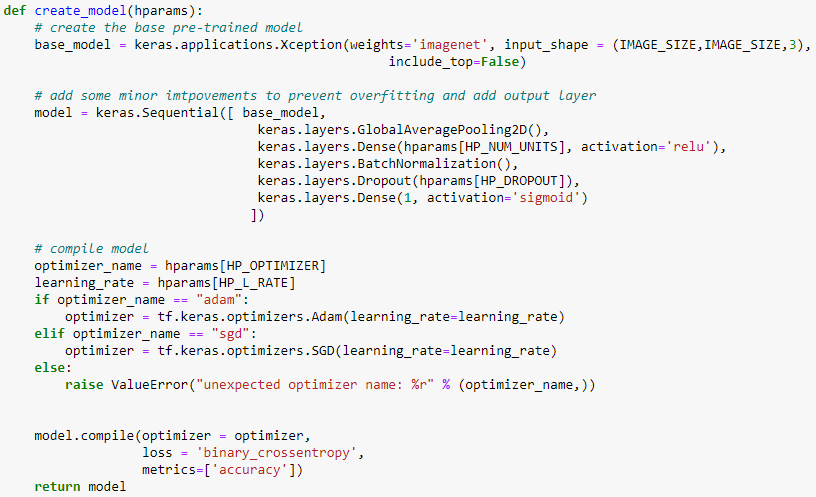
\includegraphics[width=\textwidth]{figures/xception.png}
    \caption{The create\_model() function structure, used for creating Xception in this case.}
    \label{fig:xception}
\end{figure}

While model architecture of the used models are standard, each model has been slightly modified initially for better performance, and to match the correct output specification (ie. number of classes). Each model has a different architecture and layer structure, and the following sections will explain in detail the model architecture for each, including any modifications made.

\phantomsection
\subsubsection{AlexNet}
Since Keras has no application model available for AlexNet, it had to be reproduced manually using Keras' sequential API. A description of the architecture, taken from \citep{krizhevsky2012imagenet}, was used for this.

AlexNet consists of 5 Conv2D layers, each of which is followed by a BatchNormalization layer, an Activation layer with a rectified linear activation function (ReLU) and a MaxPooling2D layer, before being passed to the next Conv2D layer. Following this the output is flattened, and passed to 3 Dense layers, each of which is followed by a BatchNormalization layer, an Activation layer with a rectified linear activation function (ReLU) and a Dropout layer. This is finally followed by an output layer, which is a Dense layer with a single output (for binary classification), a BatchNormalization layer and an Activation layer with a sigmoid activation function.

Hyper-parameter tuning involved changing the final Dense layers number of units, all three dense layers dropout values, the optimiser and the learning rate. The full model code can be seen in \autoref{fig:alexnet-part1} and \autoref{fig:alexnet-part2}.

\subsubsection{DenseNet201}


\subsubsection{ResNet50V2}


\subsubsection{SqueezeNet}


\subsubsection{Xception}


\subsubsection{ConvNet}


\subsection{Cross Validation Training}


\subsection{Model Evaluation}


\section{Operation of Artefact}

\section{Initial Results}

\section{Model Improvements}

\section{Final Results}
